\subsection{Gegensprechanlage}

Mit der Integration von synchroner Sprachübertragung wird das Praxisrufsystem um die Funktion Gegensprechanlage erweitert.
Die gewählte Technologie WebRTC erlaubt es, Sprachverbindungen zwischen Clients aufzubauen.
Dieses Kapitel beschreibt wie das Praxisrufsystem erweitert wird, um eine konfigurierbare Gegensprechanlage mit WebRTC zu implementieren.

\subsubsection{Konfiguration}

Die Gegensprechanlage wird in den nativen Mobile Client integriert.
Praxismitarbeitende können über Buttons Sprachverbindungen zu anderen Clients aufbauen.
Welche Buttons und damit welche Sprachverbindungen zur Verfügung stehen, wird durch Praxisadministrierende über das Admin UI konfiguriert.
Damit dies möglich ist, sind Änderungen an de Configuration-Modul des Cloudservice sowie am Admin UI notwendig.

Die Konfiguration von Mobile Clients wird in der Domäne Configuration abgebildet.
Zentral sind dabei die beiden Entities Client und ClientConfiguration.
Ein Client repräsentiert ein physisches Endgerät.
Eine ClientConfiguration definiert die Konfiguration eines Gerätes.

Praxisruf bietet bereits heute die Möglichkeit Buttons zu konfigurieren, über welche Benachrichtigungen versendet werden können.
Diese Buttons werden mit der Entität NotificationType konfiguriert, welche wiederum einer ClientConfiguration zugeordnet werden können.
Diese ClientConfiguration wird bei der Anmeldung auf dem Mobile Client geladen und verwendet, um die nötigen Buttons darzustellen.
Für die Konfiguration von Sprachverbindungen wird die Entität CallType erstellt.
Ein CallType beinhaltet den Text, welcher auf dem zugehörigen Button auf Clientseite angezeigt wird und eine Liste von Clients, welche als Ziel der Sprachverbindung verwendet werden.
Abbildung 7.14 zeigt einen Ausschnitt aus dem Entity Relationship Diagramm der Configuration Domäne.
Dabei sind die Teile, die für die Konfiguration von Sprachverbindungen ergänzt werden, grün markiert.

\begin{figure}[h]
    \centering
    \begin{minipage}[b]{0.7\textwidth}
        \fbox{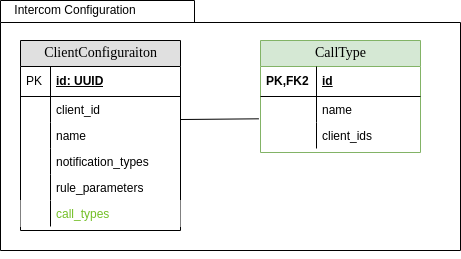
\includegraphics[width=\textwidth]{/home/joshua/FHNW/dev/IP6/IP6_Bachelorarbeit_Bericht_Cloudbasiertes_Praxisrufsystem/src/graphics/diagramms/erd_intercom_v02.drawio}}
        \caption{ERD Ausschnitt - Konfiguration Gegensprechanlage}
    \end{minipage}
\end{figure}

Das Admin UI wird mit Ansichten erweitert, über welche CallTypes erstellt, angezeigt, bearbeitet und gelöscht werden können.
Gleichzeitig wird der Cloudservice um Rest Endpunkte für das Lesen, Erstellen, Aktualisieren und Löschen von CallTypes erweitert.
Die Ansichten für ClientConfigurations im Admin UI werden so erweitert, dass CallTypes darauf angezeigt, hinzugefügt und entfernt werden können.
Die API des Cloudservice wird erweitert, um die erweiterte Konfiguration verwalten zu können.

\clearpage

\subsubsection{Signaling Instanz}

Mit WebRTC werden Peer-To-Peer Verbindungen aufgebaut~\cite{webrtc}.
Damit diese Verbindungen aufgebaut werden können, müssen die beteiligten Geräte Signalmeldungen austauschen können.
Dazu ist eine Instanz notwendig, welche Signale zwischen den Endgeräten vermitteln kann.
Diese Signaling Instanz wird als Teil des Cloudservice implementiert.

Der Cloudservice wird um ein neues Modul ''Signaling'' erweitert.
Dieses soll den Austausch von Signalen zwischen Clients ermöglichen.
Gleich wie das Modul für Sprachsynthese wird es unabhängig von den anderen Domänenmodulen im Cloudservice implementiert.
Das Modul Signaling muss dabei zwei Aufgaben übernehmen.
Erstens muss es Mobile Clients die Möglichkeit bieten, sich für Sprachverbindungen zu registrieren.
Zu diesem Zweck müssen Mobile Clients eine Verbindung mit der Signaling Instanz herstellen und trennen können.
Zweitens muss es Signalmeldungen empfangen und an die relevanten Empfänger zustellen können.
Kann eine Signalmeldung nicht zugestellt werden, muss es den betroffenen Empfänger über das verpasste Signal informieren.

Für diese Funktionen wird das Interface ClientConnector definiert.
Dieses definiert die Methoden afterConnectionEstablished und afterConnectionClosed.
Die beiden Methoden werden aufgerufen, wenn eine Verbindung geöffnet bzw.\ geschlossen wurde.
Die Implementierung dieses Interfaces ist dafür verantwortlich verfügbare Verbindungen zu verwalten.
Weiter definiert das Interface die Methode handleSignal.
Diese muss verwendet werden, um ein Signal entgegenzunehmen und an relevante Empfänger weiterzuleiten.

\begin{figure}[h]
    \centering
    \begin{minipage}[b]{1\textwidth}
        \fbox{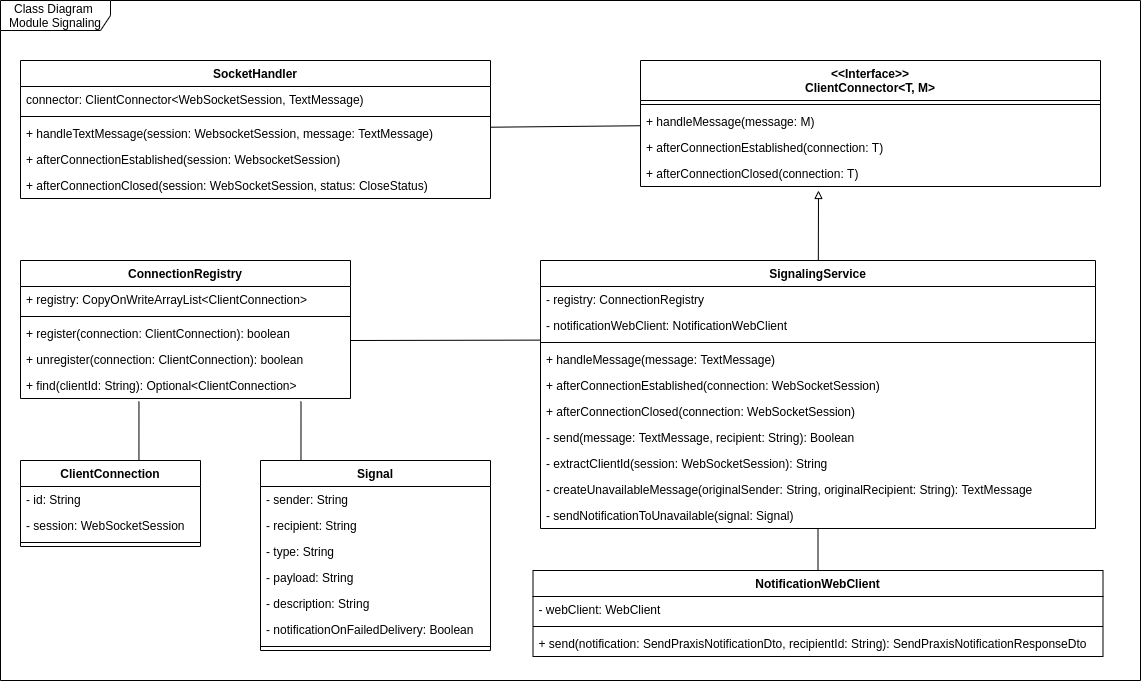
\includegraphics[width=\textwidth]{/home/joshua/FHNW/dev/IP6/IP6_Bachelorarbeit_Bericht_Cloudbasiertes_Praxisrufsystem/src/graphics/diagramms/Class_Intercom_Full_V01}}
        \caption{Klassendiagramm - Modul Signaling}
    \end{minipage}
\end{figure}

Für die Verwaltung von Verbindungen wird die Komponente ConnectionRegistry implementiert.
Diese führt eine Liste bekannter Verbindungen und bietet Methoden um Verbindungen zu registrieren und wieder entfernen.
Sie bietet weiter eine Methode, um zu überprüfen, ob eine bestimmte Verbindung bekannt ist.
Bekannte Verbindungen werden mit der Klasse ClientConnection abgebildet.
Ein ClientConnection beinhaltet immer einen Identifikator und das technische Verbindungsobjekt.
So können Verbindungen in der ClientConnection immer über einen eindeutigen Identifikator registriert und gefunden werden.

Die Klasse SignalingService implementiert das ClientConnector Interface.
Sie verwendet die Klasse ConnectionRegistry, um eine Liste von verfügbaren Verbindungen zu führen.
Über die Methoden onConnectionEstablished werden neue Verbindungen in der ConnectionRegistry registriert.
Mit der Methode onConnectionClosed werden geschlossene Verbindungen wieder entfernt.

Für das Zustellen von Signalen über bekannte Verbindungen wird die Methode handleSignal implementiert.
Jedes Signal beinhaltet die Identifikation seines Empfängers.
Beim Empfang eines Signals wird kontrolliert, ob die ConnectionRegistry eine Verbindung für die Identifikation des Empfängers enthält.
Ist dies der Fall, wird das Signal über diese Verbindung an den Empfänger übermittelt.
Wenn dies nicht der Fall ist oder wenn das Senden des Signals fehlschlägt, ist der Empfänger nicht erreichbar.
Nicht erreichbare Empfänger werden mit Benachrichtigungen über verpasste Signale informiert.
Dazu wird eine Benachrichtigung über die API des Moduls Notification versendet.

Die Schnittstelle der Signaling Instanz im Cloudservice wird mit Websockets umgesetzt.
Dazu wird die Bibliothek Spring-Boot-Starter-Websocket verwendet.
Es wird ein WebsocketHandler implementiert, welcher unter dem Pfad ''$<$serverUrl$>$/signaling'' erreichbar ist.
Etablierte Verbindungen müssen eindeutig einem Client zugeordnet werden können.
Diese Identifikation wird als Query Parameter bei Verbindungsaufbau mitgegeben.
Der WebsocketHandler definiert Methoden die beim Öffnen und Schliessen von Verbindungen sowie beim Empfang von Signalen aufgerufen werden.
Die Verarbeitung dieser Signale und Verbindungen wird an den SignalingService delegiert.

\subsubsection{Sicherheit für Signaling}

Der Zugriff auf die Signaling Instanz und die darüber ausgetauschten Signale darf nur für Berechtigte möglich sein.
Um dies sicherzustellen, wird der Verbindungsaufbau nur erlaubt, wenn die Anfrage dazu authentisiert ist.
Für die Authentisierung wird derselbe Mechanismus wie für Http-Anfragen der Cloudservice-API verwendet.
Durch die Konfiguration des Cloudservices wird die Authentifizierung aller Http Requests überprüft.
Mit dieser Prüfung wird sichergestellt, dass gültige Authentifizierungsdaten im Header der Anfrage vorhanden sind.
Ist dies nicht der Fall, wird eine entsprechende Fehlermeldung zurückgegeben.
Bei der Prüfung von Http-Anfragen durch den Cloudservice werden weiter die Rollen, welche dem Aufrufer zugeteilt sind ausgelesen.

Diese Prüfung der Authentifizierung wird auch für die Http-Anfragen, welche zum Aufbau einer Websocketverbindung nötig sind ausgeführt.
Beinhaltet eine Anfrage zum Aufbau einer Websocketverbindung keine gültige Authentifizierung, wird eine Fehlermeldung zurückgegeben.
Der Aufbau der Websocketverbindung wird abgebrochen.

Die Prüfung der ausgelesenen Rollen wird mit der Klasse HttpSessionHandshakeInterceptor implementiert.
Diese wird, nachdem eine Anfrage zum Aufbau einer Websocketverbindung eingegangen ist, aufgerufen.
Der HttpSessionHandshakeInterceptor erlaubt es die Anfrage zum Verbindungsaufbau auszulesen.
Dies erlaubt es hier zu verifizieren, dass der Request authentifiziert wurde und nur die zugeteilten Rollen zu überprüfen.
Praxisruf kennt die zwei Rollen ''ADMIN'' und ''USER''.
Beide Rollen sind berechtigt, dass Rufsystem über den Mobile Client zu verwenden und dürfen damit Signalmeldungen austauschen.
Hat der Aufrufer keine dieser Rollen, wird der Verbindungsaufbau abgebrochen.

Für Websocketverbindungen wird ausschliesslich das Protokoll Secure WebSockets (WSS) verwendet.
Die Http-Anfragen für den Verbindungsaufbau werden ausschliesslich über Https versendet.
Der Verbindungsaufbau und Austausch von Signalmeldungen über das Signaling Modul sind damit verschlüsselt.

\clearpage

\subsubsection{Anmeldung und Registrierung}

Dieses Kapitel beschreibt, welche Anmelde- und Registrierungsprozesse im Mobile Client benötigt werden.

Anmeldung und Registrierung für Benachrichtigungen funktionieren mit dem neuen Mobile Client nach demselben Ablauf wie im Vorgängerprojekt.
Die Registrierung für Sprachverbindungen beim Signaling Modul des Cloudservice wird mit diesem Projekt hinzugefügt.
Der gesamte Ablauf von Anmeldung und Registrierung wird in Abbildung 7.16 dargestellt.
Praxismitarbeitende öffnen die Applikation und geben ihr Benutzername und Passwort ein.
Der Mobile Client verwendet diese, um sich über Basic Authentication beim Cloudservice anzumelden.
Als Antwort auf die Anmeldung gibt der Cloudservice ein Json Web Token (JWT) zurück.
Dieses wird lokal auf dem Gerät gespeichert und für alle weiteren Anfragen an den Cloudservice verwendet.
Nachdem die Anmeldung erfolgt ist, wird eine Liste der verfügbaren Konfigurationen geladen.
Der Benutzer wählt die gewünschte Konfiguration aus und bestätigt.

\begin{figure}[h]
    \centering
    \begin{minipage}[b]{0.9\textwidth}
        \fbox{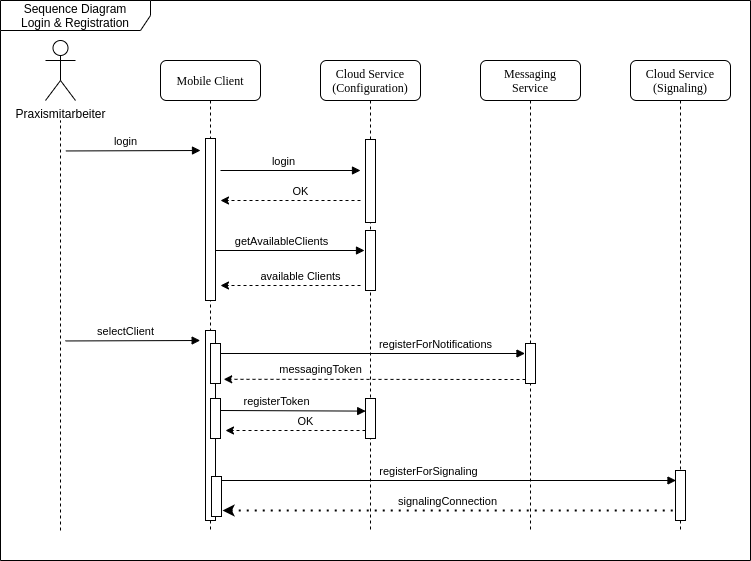
\includegraphics[width=\textwidth]{/home/joshua/FHNW/dev/IP6/IP6_Bachelorarbeit_Bericht_Cloudbasiertes_Praxisrufsystem/src/graphics/diagramms/Sequence_Registration}}
        \caption{Sequenzdiagramm - Anmeldung und Registrierung im Mobile Client}
    \end{minipage}
\end{figure}

Danach wird diese Konfiguration geladen und die Hauptansicht angezeigt.
Die geladene Konfiguration beinhaltet alle Informationen die nötig sind um Buttons für Benachrichtigungen und Sprachverbindungen anzuzeigen.
Im Hintergrund muss sich der Mobile Client nun für Benachrichtigungen und Sprachverbindungen registrieren.
Für Benachrichtigungen registriert er sich zuerst bei Firebase Cloud Messaging.
Er erhält ein Token, welches den Client beim Messaging Service identifiziert.
Dieses Token sendet der Mobile Client zusammen mit der gewählten Konfiguration an den Cloudservice.
Dieser persistiert die Registrierung und kann sie verwenden, um Benachrichtigungen an diesen Client zuzustellen.
Für Sprachverbindungen muss zudem eine Verbindung zum Signaling Modul des Cloudservices aufgebaut werden.
Dazu wird wie in Kapitel 7.4.6 beschrieben eine Websocketverbindung geöffnet.

\clearpage

\subsubsection{Signalmeldungen}

Dieses Kapitel beschreibt die Signalmeldungen, welche in Praxisruf verwendet werden.
Dabei wird beschrieben wie diese aufgebaut sind und welchen Rolle sie im System erfüllen.
Abbildung 7.17 zeigt, wie Signalmeldungen im Mobile Client modelliert werden.

\begin{figure}[h]
    \centering
    \begin{minipage}[b]{0.5\textwidth}
        \fbox{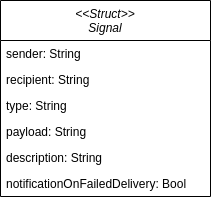
\includegraphics[width=\textwidth]{graphics/diagramms/Class_Signal}}
        \caption{Klassendiagramm - Signal}
    \end{minipage}
\end{figure}

Alle Signalmeldungen beinhalten Identifikation von Sender und Empfänger.
Diese werden von der Signaling Instanz verwendet, um die Signale korrekt weiterzuleiten.
Die Werte Type, Payload und Description werden im Mobile Client verwendet, um das Signal korrekt zu verarbeiten und Verbindungen aufzubauen.
Das Flag notificationOnFailedDelivery wird im Cloudservice ausgewertet.
Wenn ein Signal nicht zugestellt werden kann und dieses Flag aktiviert ist, wird der Empfänger mit einer Benachrichtigung darüber informiert.
Dazu wird die API des Notification Moduls des Cloudservices verwendet.

Praxisruf verwendet sechs Typen von Signalmeldungen.
Folgende Übersicht beschreibt pro Typ welche Daten ein Signal beinhaltet und welche Rolle es erfüllt.
\\
\begin{tabbing}
    Left \= Middle \= Right \= Right \kill
    Offer
    \> \> \> Wird vom Initiator der Sprachverbindung an die Empfänger gesendet. Ein Offer
    \\\> \> \> beinhaltet die SDP Informationen des Initiators und initiiert eine Verbindung. \\ \\

    Answer
    \> \> \> Wird vom Empfänger eines Offers an den Initiator der Sprachverbindung gesendet.
    \\\> \> \> Es beinhaltet SDP Informationen des Empfängers und bestätigt eine Verbindung. \\ \\

    Ice Candidate
    \> \> \> Beinhaltet Informationen eines ICE Candidates, die für den Verbindungsaufbau ver-
    \\ \> \> \> wendet werden. Nach Verarbeitung von Offer und Answer tauschen Initiator und
    \\ \> \> \> Empfänger solange Ice Candidate Signale aus, bis sie sich auf einen Kandidaten
    \\ \> \> \> geeinigt haben. Dieser wird verwendet, um die Verbindung aufzubauen.
    \\ \> \> \> \\

    End
    \> \> \> Wird versendet, nachdem die Verbindung durch tippen des Auflegen-Button in der
    \\ \> \> \> Applikation beendet wurde. Empfang dieses Signal führt dazu, dass offene Sprach-
    \\ \> \> \> verbindungen zum Sender dieses Signals beim Empfänger beendet werden.\\ \\

    Unavailable
    \> \> \> Wenn der Signalingserver ein Signal nicht zustellen kann, wird ein Unavailable-
    \\ \> \> \> Signal zurück an den Sender gesendet. Der Sender ist so informiert, dass die Ver-
    \\ \> \> \> bindung zum Gesprächspartner nicht aufgebaut wurde. \\ \\

    Decline
    \> \> \> Wird ein Offer empfangen während die Gegensprechanlage in den lokalen Einstel-
    \\ \> \> \> lungen deaktiviert ist oder bereits in Anruf aktiv ist, sendet der Mobile Client ein
    \\ \> \> \> Decline Signal zurück. Der Sender ist so informiert, dass die Verbindung zum Ge-
    \\ \> \> \> sprächspartner abgelehnt wurde.
\end{tabbing}

\clearpage

\subsubsection{Verbindungsaufbau}

Praxismitarbeitende können Sprachverbindungen zu anderen Clients aufbauen indem sie auf den entsprechenden Button in der Praxisruf App tippen.
Zum Zeitpunkt an dem der Button getippt wird, weiss der Mobile Client noch nicht, zu welchen Clients diese Verbindung aufgebaut werden soll.
Als Erstes muss deshalb beim Cloudservice angefragt werden, zu welchen Clients eine Sprachverbindung aufgebaut werden soll.
Der Cloudservice bietet dazu einen Endpoint an, über den der vollständige CallType des verwendeten Buttons geladen werden kann.
Nachdem diese Informationen geladen sind, können Sprachverbindungen zu allen Empfängern aufgebaut werden.
Dazu müssen Offer, Answer und Ice Candidate Signale ausgetauscht werden.
Der auslösende Client initialisiert die Peer-to-Peer Verbindung auf seiner Seite und sendet für jeden Gesprächspartner ein Offer.
Der Cloudservice findet die Verbindung der jeweiligen Empfänger und leitet die Signale über deren Verbindung weiter.

Nach Eingang des Offer-Signals wird die Verbindung auf Empfängerseite initialisiert und eine Answer zurück an den Initiator gesendet.
Diese wird gleich wie das Offer-Signal über die Signaling Instanz zugestellt.
Der Initiator empfängt die Antwort Signale und ergänzt die notwendigen Verbindungsinformationen.
Abbildung 7.18 visualisiert diesen Ablauf.

\begin{figure}[h]
    \centering
    \begin{minipage}[b]{0.9\textwidth}
        \fbox{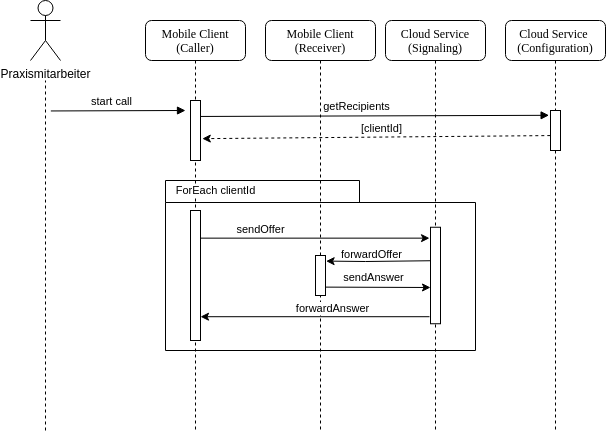
\includegraphics[width=\textwidth]{graphics/diagramms/Sequence_Intercom_Broking_V02}}
        \caption{Sequenzdiagramm - Verbindungsaufbau mit Offer und Answer Signalen}
    \end{minipage}
\end{figure}

Nachdem die Offer und Answer Meldungen ausgetauscht sind, müssen Ice Candidate Meldungen ausgetauscht werden.
Der Austausch von Ice Candidate Meldungen wird so lange wiederholt, bis sich beide Seiten einer Verbindung auf Verbindungsdetails geinigt haben.
Sobald dieser Austausch beendet ist, besteht die Verbindung und es können Sprachdaten ausgetauscht werden.

\clearpage

\subsubsection{Anbindung Mobile Client an Singaling Instanz}

Dieses Kapitel beschreibt, wie Websockeverbindungen zum Austausch von Signalmeldungen in den nativen Mobile Client integriert werden.

In Kapitel 7.2 wird die Klasse PraxisrufApi beschrieben.
Diese implementiert die Anbindung and die Http-API des Cloudservice.
Um Signalmeldungen über die Signaling Instanz des Cloudservice auszutauschen, müssen Websockets verwendet werden.
Damit die Anbindung an alle Schnittstellen des Cloudservice einheitlich bleibt, wird PraxisrufApi erweitert, um auch Websocketverbindungen zu unterstützen.
Dies beinhaltet den Auf- und Abbau von Verbindungen, sowie das Senden und Empfangen von Meldungen über diese Verbindung.
Weiter müssen Verhalten beim Empfang von Fehlermeldungen und dem unerwarteten Schliessen der Verbindung definiert werden.

Der Austausch von Signalmeldungen ist der einzige Anwendungsfall für Websockets in Praxisruf.
Deshalb wird auf eine generische Integration von Websockets verzichtet.
Zur Erweiterung von PraxisrufApi werden die Extension PraxisrufApi+Signaling und das Protokoll PraxisrufApiSignalingDelegate definiert.
Diese setzen die Anbindung von Websockets für den Austausch von Signalmeldungen um.

\begin{figure}[h]
    \centering
    \begin{minipage}[b]{0.6\textwidth}
        \fbox{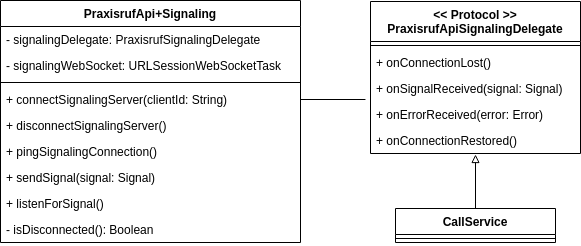
\includegraphics[width=\textwidth]{graphics/diagramms/Class_Mobile_Client_Signaling_Connection}}
        \caption{Klassendiagramm - Signaling Schnittstelle in Mobile Client}
    \end{minipage}
\end{figure}

Die Extension PraxisrufApi+Signaling ist für die Verbindung zu der Signaling Instanz verantwortlich.
Für die Integration dieser Extension in den Rest der Applikation wird das Protokoll PraxisrufApiSignalingDelegate definiert.
Zum Aufbau der Verbindung zu der Signaling Instanz wird die Methode connectSignalingServer definiert.
Die Identifikation des Clients wird bei dieser Abfrage als Parameter mitgegeben.
So kann die Verbindung von der Signaling Instanz eindeutig einem Client zugeordnet werden.
Nachdem die Verbindung geöffnet ist, können Signale empfangen und verarbeitet werden.
Dies wird durch die Methode listenForSignal initialisiert.
Darin wird der Websocketverbindung signalisiert, dass der Client bereit ist die nächste Meldung zu empfangen.
Sobald eine Meldung empfangen wird, wird diese über den PraxisrufApiSignalingDelegate verarbeitet.
Wurde eine gültige Signalmeldung empfangen, wird diese über die Methode onSignalReceived verarbeitet.
Wurde hingegen eine ungültige Signalmeldung oder eine Fehlermeldung empfangen wird die Methode onErrorReceived aufgerufen.
Im Fehlerfall wird zudem überprüft, ob die Verbindung noch offen verwendbar ist.
Sollte die Verbindung nicht mehr verwendbar sein, wird die Methode onConnectionLost des Delegates aufgerufen.
Dadurch wird versucht, die Verbindung erneut aufzubauen.
Ist dies nicht möglich, wird eine Fehlermeldung angezeigt. 

PraxisrufApi+Signaling definiert weiter Methoden um Signal- und Pingmeldungen zu versenden.
Pingmeldungen werden in Regelmässigen Abständen gesendet um sicherzustellen, dass die Verbindung zu der Signaling Instanz geöffnet bleibt.
Vor dem Senden jeder Meldung wird geprüft, ob die Verbindung zur Signaling Instanz verwendbar ist.
Ist dies nicht der Fall, wird die Methode onConnectionLost des Delegates aufgerufen und anschliessend versucht die Meldung zu versenden.
Schlägt das Senden fehl, wird die Methode onErrorReceived auf dem Delegate aufgerufen.

Die Methoden des Protokolls CallClientDelegate werden durch die Klasse CallService implementiert.
Der CallService vermittelt Anfragen zwischen Signaling Instanz, Benutzeroberfläche und Peer-To-Peer Verbindungen im Mobile Client.
Er ist dafür verantwortlich Signale an die Peer-To-Peer Verbindung weiterzuleiten, geschlossene Verbindungen wieder zu öffnen und Fehlermeldungen anzuzeigen.
Empfangene Signalmeldungen werden über die Methode onSignalReceived an die Komponente CallClient übergeben (Siehe Kapitel 7.4.9).
Die Methoden onConnectionLost und onErrorReceived werden verwendet, um Fehlermeldungen anzuzeigen und geschlossene Verbindungen erneut zu öffnen.
Nachdem die Verbindung zur Signaling Instanz verloren gegangen ist, wird bis zu zehnmal versucht, die Verbindung erneut zu öffnen.
Wenn die Verbindung dadurch nicht repariert werden kann, wird sie geschlossen und dem Benutzer eine Fehlermeldung angezeigt.

\subsubsection{Verbindungsverwaltung}

Dieses Kapitel beschreibt, wie im Mobile Client sichergestellt wird, dass die Verbindung zu der Signaling Instanz langfristig zur Verfügung steht.
Abbildung 7.20 gibt einen Überblick, über die Abläufe dazu umgesetzt werden.
Dieser Ablauf ist mit den Komponenten CallService und PraxisrufApi+Signaling die, in Kapitel 7.4.7 beschrieben sind, implementiert.

\begin{figure}[h]
    \centering
    \begin{minipage}[b]{1\textwidth}
        \fbox{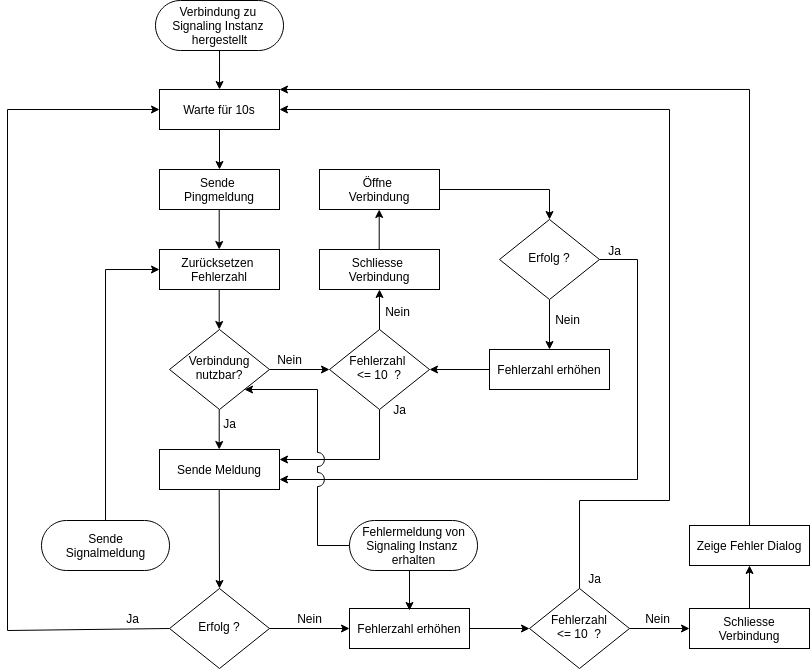
\includegraphics[width=\textwidth]{graphics/diagramms/flow_connection}}
        \caption{Flowchart - Verbindungsverwaltung}
    \end{minipage}
\end{figure}

Um festzustellen, ob die eine getrennte Verbindung repariert werden kann, wird im CallService ein Fehlerzähler geführt.
Dieser wird beim Start der Applikation mit null initialisiert und bei jedem Verbindungsfehler um eins inkrementiert.
Ein Verbindungsfehler tritt auf, wenn eine Fehlermeldung über die Signaling Verbindung empfangen wird und wenn das Senden einer Meldung oder das Wiederherstellen der Verbindung fehlschlägt.

Die Verbindung zur Signaling Instanz wird hergestellt, sobald die Applikation gestartet wird.
Nachdem die Verbindung hergestellt wurde, werden im Abstand von zehn Sekunden Pingmeldungen über die Verbindung gesendet.
Dadurch wird sichergestellt, dass die Verbindung geöffnet bleibt.
Vor dem Versenden jeder Meldung wird der Fehlerzähler zurückgesetzt und es wird überprüft, ob die Verbindung verwendet werden kann.
Ist die Verbindung fehlerhaft, werden bis zu zehn Versuche unternommen, sie wiederherzustellen.
Anschliessend wird versucht, die Meldung zu versenden.
Wenn die Meldung erfolgreich versendet wurde, wird der Fehlerzähler zurückgesetzt und zehn Sekunden gewartet, bis die nächste Pingmeldung versendet wird.
Andernfalls wird die Fehlerzahl um eins erhöht.
Ist die Fehlerzahl danach grösser als zehn, wird die Verbindung getrennt.
In der Benutzeroberfläche wird ein Fehlerdialog angezeigt.
Die Verbindung bleibt geschlossen bis die nächste Meldung versendet wird.
Dies der Fall, wenn das Interval für die nächste Pingmeldung abgelaufen ist oder wenn ein Anruf über die Benutzeroberfläche gestartet wird.

Bei Start eines Anrufes aus der Benutzeroberfläche werden dieselben Prüfungen, wie vor dem Versenden von Pingmeldungen ausgeführt.
So werden geschlossene Verbindungen zur Signaling Instanz frühzeitig repariert.
Weiter wird nach Empfang jedes Fehlers über die Signaling Verbindung geprüft, ob diese noch offen ist.
Ist dies nicht der Fall, werden auch hier bis zu zehn Versuche unternommen, die Verbindung wiederherzustellen.

Dieser Ablauf stellt sicher, dass die Verbindung zu der Signaling Instanz geöffnet bleibt und wenn nötig repariert wird.
Wenn möglich, geschieht dies direkt nach Verbindungsverlust.
Andernfalls werden Praxismitarbeitende informiert, dass die Verbindung nicht hergestellt werden konnte.
Im Hintergrund wird in dieser Situation regelmässig versucht, die Verbindung zu reparieren.
Die Bedienelemente für die Gegensprechanlage bleiben während dieser Zeit aktiviert und können weiter verwendet werden.
Wenn Praxismitarbeitende einen Anruf starten und die Verbindung immer noch getrennt ist, wird die sie frühzeitig wiederhergestellt.
Ist dies erfolgreich, wird der Anruf gestartet.
Andernfalls wird erneut ein Fehlerdialog angezeigt.

\clearpage

\subsubsection{Sprachverbindungen im Mobile Client}

Dieses Kapitel beschreibt wie WebRTC-Komponenten in den Mobile Client integriert werden, um Sprachverbindungen zu ermöglichen.

Für die Integration der WebRTC-Komponenten wird eine Klasse CallClient und ein Protokoll CallClientDelegate erstellt.
Der CallClient verwaltet Sprachverbindungen, während der Delegate zur Integration mit der restlichen Applikation dient.
Abbildung 7.21 zeigt das Klassendiagramm beider Komponenten.
Die Methoden des CallClientDelegate-Protokolls werden von der Klasse CallService implementiert.
Da diese Klasse auch das Protokoll SignalingDelegate implementiert, kann sie verwendet werden um Signalmeldungen zwischen CallClient und PraxusrufApi+Signaling zu vermitteln.

\begin{figure}[h]
    \centering
    \begin{minipage}[b]{0.6\textwidth}
        \fbox{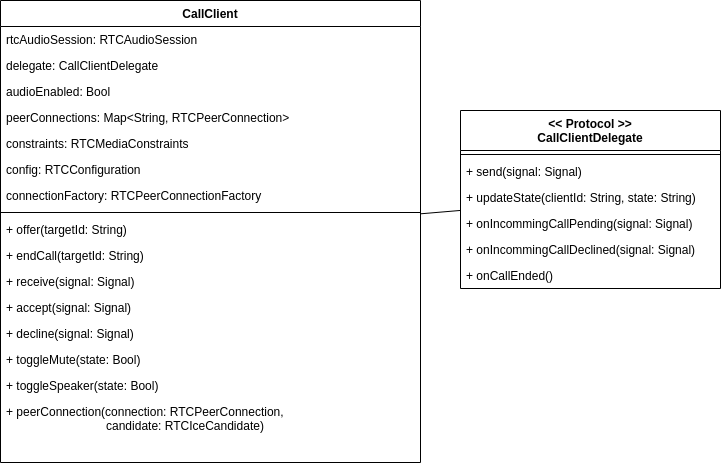
\includegraphics[width=\textwidth]{graphics/diagramms/Class_Mobile_Client_Signal_Processing}}
        \caption{Klassendiagramm - CallClient und CallClientDelegate}
    \end{minipage}
\end{figure}

Für den Aufbau von ausgehenden Verbindungen wird eine RTCPeerConnection im CallClient des Senders initialisiert.
Es werden die SDP Informationen für Beschreibung der Verbindung erstellt und mit einem Offer-Signal an den Empfänger gesendet.
Dieses Offer-Signal wird über den CallClientDelegate versendet, welcher das Signal an die Signaling Instanz zustellt.

Für den Aufbau von eingehenden Verbindungen wird das Offer-Signal über die Methode receive empfangen.
Dabei wird die Verbindung nicht direkt initialisiert.
Stattdessen wird das Signal zwischengespeichert und die Methode onIncommingCallPending des Delegates aufgerufen.
Die Implementation des CallClientDelegate navigiert darauf zu der Ansicht für aktive Anrufe und meldet dem CallClient über die Methode acceptPending, dass die Verbindung initialisiert werden soll.
Der CallClient initialisiert darauf eine RTCPeerConnection und sender ein Answer Signal über die send Methode.

Answer-Signal werden ebenfalls über die receive Methode im CallClient empfangen.
Beim Empfang einer Answer werden die SDP Informationen auf der lokalen RTCPeerConnection ergänzt.

Neben dem Austausch von Offer- und Answer-Signalen müssen Ice Candidate Signale ausgetauscht werden können.
Sobald ein Ice Candidate zur Verfügung steht, erstellt der CallClient ein entsprechendes Signal und sendet es an den Empfänger.
Damit dies möglich ist, muss der CallClient über verfügbare Ice Candidates informiert werden.
Die WebRTC Bibliothek bietet dazu das Protokoll RTCPeerConnectionDelegate.
Dieses kann auf der RTCPeerConnection registriert werden und wird aufgerufen, sobald ein neuer Ice Candidate verfügbar ist.
Der CallClient implementiert dieses Protokoll und registriert sich auf allen RTCPeerConnections.

Sprachverbindungen müssen über die Benutzeroberfläche verwaltet werden können.
Der CallClient bietet deshalb Methoden an, um eine Verbindung zu starten und beenden.
Weiter bietet er die Möglichkeit Mikrofon und Lautsprecher für geöffnete Verbindungen stummzuschalten.
Bei eingehenden Verbindungen, dem Beenden von Anrufen und Veränderungen am Status einer Verbindung, muss die Benutzeroberfläche informiert werden.
Der CallClientDelegate definiert dazu Methoden über welche der CallClient diese Informationen weitergeben kann.

\subsubsection{Signalverarbeitung im Mobile Client}

Peer-To-Peer Sprachverbindungen werden über die Komponenten CalService, CallClient und PraxisrufApi+Signaling in den Mobile Client integriert.
Dieses Kapitel beschreibt den Kommunikationsablauf zwischen diesen Komponenten anhand des Austauschs von Offer- und Answer-Signalen.

\begin{figure}[h]
    \centering
    \begin{minipage}[b]{0.85\textwidth}
        \fbox{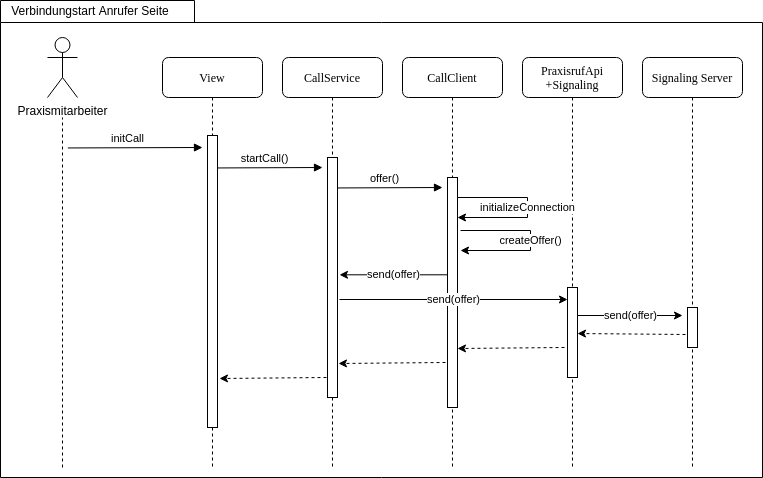
\includegraphics[width=\textwidth]{/home/joshua/FHNW/dev/IP6/IP6_Bachelorarbeit_Bericht_Cloudbasiertes_Praxisrufsystem/src/graphics/diagramms/Sequence_MobileClient_Caller_Signaling.drawio}}
        \caption{Sequenzdiagramm - Initialisierung Sprachverbindung auf Senderseite }
    \end{minipage}
\end{figure}


Die Klassen CallClient und PraxisrufApi+Signaling definieren je ein Delegate-Protokoll.
Diese Protokolle definieren die Funktionen, über welche die Komponenten Informationen weitergeben können.
Die Klasse CallService implementiert beide Delegate-Protokolle.
Er erstellt Instanzen von CallClient und PraxisrufApi+Signaling und registriert sich anschliessend bei beiden als Delegate.
Der CallService selbst wird in den View Komponenten der Applikation verwendet.
Er nimmt Benutzereingaben entgegen und delegiert die entsprechende Funktionalität an den CallClient und PraxisrufApi+Signaling.
Er nimmt ausserdem Informationen von CallClient und Signaling entgegen und stellt Anzeigeinformationen für die Benutzeroberfläche zur Verfügung.

Abbildung 7.22 zeigt die Kommunikation zwischen den beteiligten Komponenten bei der Initialisierung einer Sprachverbindung auf Empfängerseite.
Dabei wird der Ablauf von Benutzerinteraktion des Senders bis zum Senden des Offer-Signals dargestellt.
Sobald Praxismitarbeitende einen Anruf startet, wird die View für aktive Anrufe geladen.
Diese initialisiert den Anruf über den CallService.
Der CallService ruft dazu als Erstes den CallClient auf.
Der CallClient initialisiert die lokalen Verbindungsinformationen und erstellt ein Signal, um den Empfänger zu informieren.
Dieses Signal gibt er an den CallService weiter.
Der CallService leitet das Signal an den PraxisrufApi+Signaling weiter, welcher das Versenden an den Cloudservice übernimmt.

\begin{figure}[h]
    \centering
    \begin{minipage}[b]{0.85\textwidth}
        \fbox{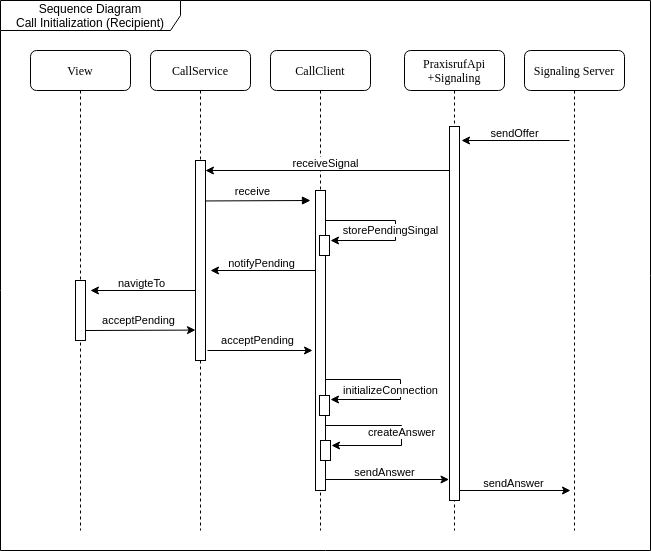
\includegraphics[width=\textwidth]{/home/joshua/FHNW/dev/IP6/IP6_Bachelorarbeit_Bericht_Cloudbasiertes_Praxisrufsystem/src/graphics/diagramms/Sequence_MobileClient_Receiver_Signaling.drawio.png}}
        \caption{Sequenzdiagramm - Initialisierung Sprachverbindung auf Empfängerseite }
    \end{minipage}
\end{figure}


Abbildung 7.23 zeigt den Ablauf bei Eingang eines Answer-Signals auf Empfängerseite.
Das versendete Signal wird über das Signaling Modul des Cloudservice an den Empfänger übermittelt.
Dieser empfängt das Signal über die Komponente PraxisrufApi+Signaling.
Diese gibt das Signal über die Methode onSignalReceived an den CallService weiter.
Der CallService aktiviert die Ansicht für aktive Anrufe und leitet das Signal an den CallClient weiter.
Der CallClient initialisiert die Peer-To-Peer Verbindung und erstellt ein Answer-Signal zur Bestätigung.
Dieses Signal wird wiederum über den CallService zum PraxisrufApi+Signaling weiter zum Cloudservice versendet.


\subsubsection{Netzwerkvoraussetzungen}

Praxisruf ist darauf ausgelegt innerhalb von Arztpraxen verwendet zu werden.
Dabei wird pro Zimmer ein Gerät installiert, welches als Endpunkt für das System dient~\cite{aufgabenstellung}.
Damit werden alle Endgeräte einer Praxis innerhalb der Praxis betrieben.
Dies erlaubt es, die Geräte im selben lokalen Netzwerk zu betreiben.
Ist diese Voraussetzung gegeben, kann der Verbindungsaufbau vereinfacht werden.
Da die Geräte direkt im lokalen Netzwerk kommunizieren können ist es nicht nötig, die Protokolle STUN oder TURN zu verwenden.
Damit wird es möglich auf den Betrieb eines ICE Servers zu verzichten.
Die Geräte können ICE Kandidaten für direkte Kommunikation im lokalen Netzwerk austauschen.

Die Integration von WebRTC in der iOS App wird unter der Voraussetzung umgesetzt, dass alle beteiligten Geräte im selben Netzwerk betrieben werden.
Dies vereinfacht den Aufbau von Verbindungen und erlaubt es, neben der Signaling Instanz keine weitere Infrastruktur betreiben zu müssen.
Sprachverbindungen mit Praxisruf sind deshalb nur möglich, wenn die beteiligten Geräte im selben lokalen Netzwerk betrieben werden.
Das Versenden und Empfangen von Benachrichtigungen funktioniert wie im Vorgängerprojekt auch ausserhalb des lokalen Netzwerkes.
Damit können auch für Empfänger, die nicht im lokalen Netzwerk sind, über verpasste Anrufe mit Benachrichtigungen informiert werden.

\clearpage
